\documentclass[a4paper, 14pt]{extarticle}%тип документа

%Русский язык
\usepackage[T2A]{fontenc} %кодировка
\usepackage[utf8]{inputenc} %кодировка исходного кода
\usepackage[english,russian]{babel} %локализация и переносы

%отступы 
\usepackage[left=2cm,right=2cm,top=2cm,bottom=3cm,bindingoffset=0cm]{geometry}

%Вставка картинок
\usepackage{graphicx}
\usepackage{wrapfig, caption}
\graphicspath{}
\DeclareGraphicsExtensions{.pdf,.png,.jpg, .jpeg}
\newcommand\ECaption[1]{%
     \captionsetup{font=footnotesize}%
     \caption{#1}}

%Таблицы
\usepackage[table,xcdraw]{xcolor}
\usepackage{booktabs}

%Графики
\usepackage{pgfplots}
\pgfplotsset{compat=1.9}

%Математика
\usepackage{amsmath, amsfonts, amssymb, amsthm, mathtools}

%Заголовок
\author{Подлесный Артём \\ группа 827}
\title{Работа 4.4.1 \\ ИЗУЧЕНИЕ ДИФРАКЦИОННОЙ
РЕШЁТКИ С ПОМОЩЬЮ ГОНИОМЕТРА}

\begin{document}
\maketitle

\paragraph*{Цель работы:} знакомство с работой гониометра и определение спектральных характеристик амплитудной решетки.
\paragraph*{Оборудование:} ртутная лампа, гониометр, амплитудная
и фазовая дифракционные решётки, плоскопараллельная стеклянная
пластинка, призменный уголковый отражатель, щель с микрометрическим винтом.

\section*{Краткая теория}

\begin{wrapfigure}{r}{0.3\textwidth}
\begin{center}
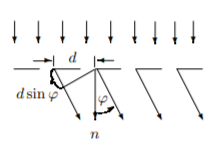
\includegraphics[height=4cm]{teor1.png}
\end{center}
\ECaption{Дифракция световых волн на дифракционной решетке.}
\end{wrapfigure}

Интенсивность дифрагированного света максимальна для углов $\varphi_m$, для которых волны, приходящие в точку наблюдения от всех
щелей решётки, оказываются в фазе.
Как следует из рис. 1, для этих направлений справедливо соотношение:
\begin{equation}
d\sin \varphi_m = m\lambda.
\end{equation}

Рассмотрим основные
характеристики дифракционной решётки.
Угловая дисперсия. Дисперсия $D$
характеризует угловое расстояние
между близкими спектральными линиями:
\[D = \dfrac{d\varphi}{d\lambda}.\]
Получаем:
\begin{equation}
D = \dfrac{m}{d\cos\varphi} = \dfrac{m}{\sqrt{d^2 - m^2\lambda^2}}.
\end{equation}

Дисперсия возрастает с увеличением порядк
а спектра. На опыте дисперсию решётки определяют путём измерения углового расстояния $\Delta\varphi$ между двумя близкими спектральными линиями с известной разностью
длин волн $ \Delta\lambda $ (например, между
жёлтыми линиями ртути).

\begin{wrapfigure}{l}{0.3\textwidth}
\begin{center}
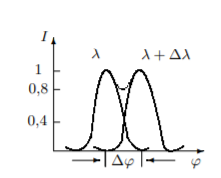
\includegraphics[height=4cm]{teor2.png}
\end{center}
\ECaption{Определение разрешающей способности дифракционной решетки.}
\end{wrapfigure}

Разрешающая способность дифракционной решётки. Возможность разрешения двух близких спектральных линий зависит от их ширины и от расстояния между ними.
Пусть в спектре
m-го порядка наблюдаются две близкие спектральные линии с длинами волн
$ \lambda $ и $ (\lambda + \Delta\lambda) $. Угловое расстояние
$ \Delta\varphi $ между этими линиями равно:
\begin{equation}
\Delta\varphi = \dfrac{m\Delta\lambda}{d\cos \varphi}.
\end{equation}
Согласно критерию разрешения
Релея линии становятся неразличимыми,
когда расстояние между ними меньше,
чем расстояние от максимума одной линии до её первого минимума (рис. 2). Угловая полуширина главного максимума равна:
\begin{equation}
\delta\varphi = \dfrac{\lambda}{Nd\cos \varphi}.
\end{equation}
По определению разрешающая способность спектрального прибора
$ R = \lambda/\delta\lambda $
— это отношение длины волны
к
разности длин волн двух
линий,
разрешаемых по критерию
Релея. Приравнивая $ \delta\varphi $
и
$ \Delta\varphi $ для
случая предельного разрешения, найдём для дифракционной решётки:
\begin{equation}
R = \dfrac{\lambda}{\delta\lambda} = mN.
\end{equation}

\section*{Экспериментальная установка.}

\begin{figure}[h!]
\begin{center}
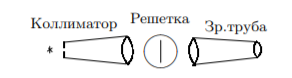
\includegraphics[width=0.6\textwidth]{ust}
\end{center}
\ECaption{Схема экспериментальной установки. В работе определялись спектральные характеристики амплитудной решетки. Известно справочное значение периода решетки: $ d = 2000 $ нм.}
\end{figure}

\section*{Исследование спектра ртутной лампы}
\subsection*{Определение периода решетки}

После длительной тонкой настройки, а так же качественной проверки того факта, что $ d\sin\varphi_m \sim\lambda $, можно приступать к наблюдению спектра. 

Для экспериментального определения периода решетки, были сняты угловые координаты полос спектра в $ \pm 1 $ порядке. результаты представлены на таблице, полосы промаркированы по своим видимым цветам.

\begin{table}[h!]
\begin{center}
\begin{tabular}{|
>{\columncolor[HTML]{9698ED}}c |c|c|c|
>{\columncolor[HTML]{9698ED}}c |c|c|c|}
\hline
\cellcolor[HTML]{6665CD}1 & \cellcolor[HTML]{9698ED}г & \cellcolor[HTML]{9698ED}м & \cellcolor[HTML]{9698ED}с & \cellcolor[HTML]{6665CD}-1 & \cellcolor[HTML]{9698ED}г & \cellcolor[HTML]{9698ED}м & \cellcolor[HTML]{9698ED}с \\ \hline
фиолет                    & 167                       & 17                        & 53                        & фиолет                     & 192                       & 37                        & 11                        \\ \hline
синий                     & 165                       & 36                        & 20                        & синий                      & 194                       & 13                        & 44                        \\ \hline
зеленый                   & 163                       & 55                        & 41                        & зеленый                    & 195                       & 48                        & 22                        \\ \hline
желтый1                   & 162                       & 58                        & 11                        & желтый1                    & 196                       & 42                        & 4                         \\ \hline
желтый2                   & 162                       & 54                        & 26                        & желтый2                    & 196                       & 46                        & 7                         \\ \hline
красный1                  & 162                       & 1                         & 35                        & красный1                   & 197                       & 44                        & 8                         \\ \hline
красный2                  & 161                       & 31                        & 14                        & красный2                   & 198                       & 33                        & 41                        \\ \hline
\end{tabular}
\ECaption{Угловые координаты разноцветных полос спектра ртутной лампы. Измерения начинаются со 180 градусов, буквы означают соответственно градусы, минуты и секунды.}
\end{center}
\end{table}

По полученным данным построен график зависимости $\lambda(\sin \varphi_n)$ на рис 4, по которому можно определить период решетки d как коэффициент наклона прямой. Зависимость цвета полосы спектра ртутной лампы от длины волны света (справочная), отражена на таблице 2.

\begin{table}[h!]
\begin{center}

\begin{tabular}{|c|c|c|c|c|c|c|c|}
\hline
\rowcolor[HTML]{9698ED} 
цвет          & фиолет & синий & зеленый & желтый1 & желтый2 & красный1 & красный2 \\ \hline
$\lambda$, нм & 404.7  & 435.8 & 546.1   & 577     & 579.1   & 623.4    & 690.7    \\ \hline
\end{tabular}
\ECaption{Cопоставление цвета полосы и длины волны света. В спектре так же планировалось наблюдать голубую полосу, однако её так и не удалось увидеть.}
\end{center}
\end{table}
       
\begin{figure}[h!]
\begin{center}
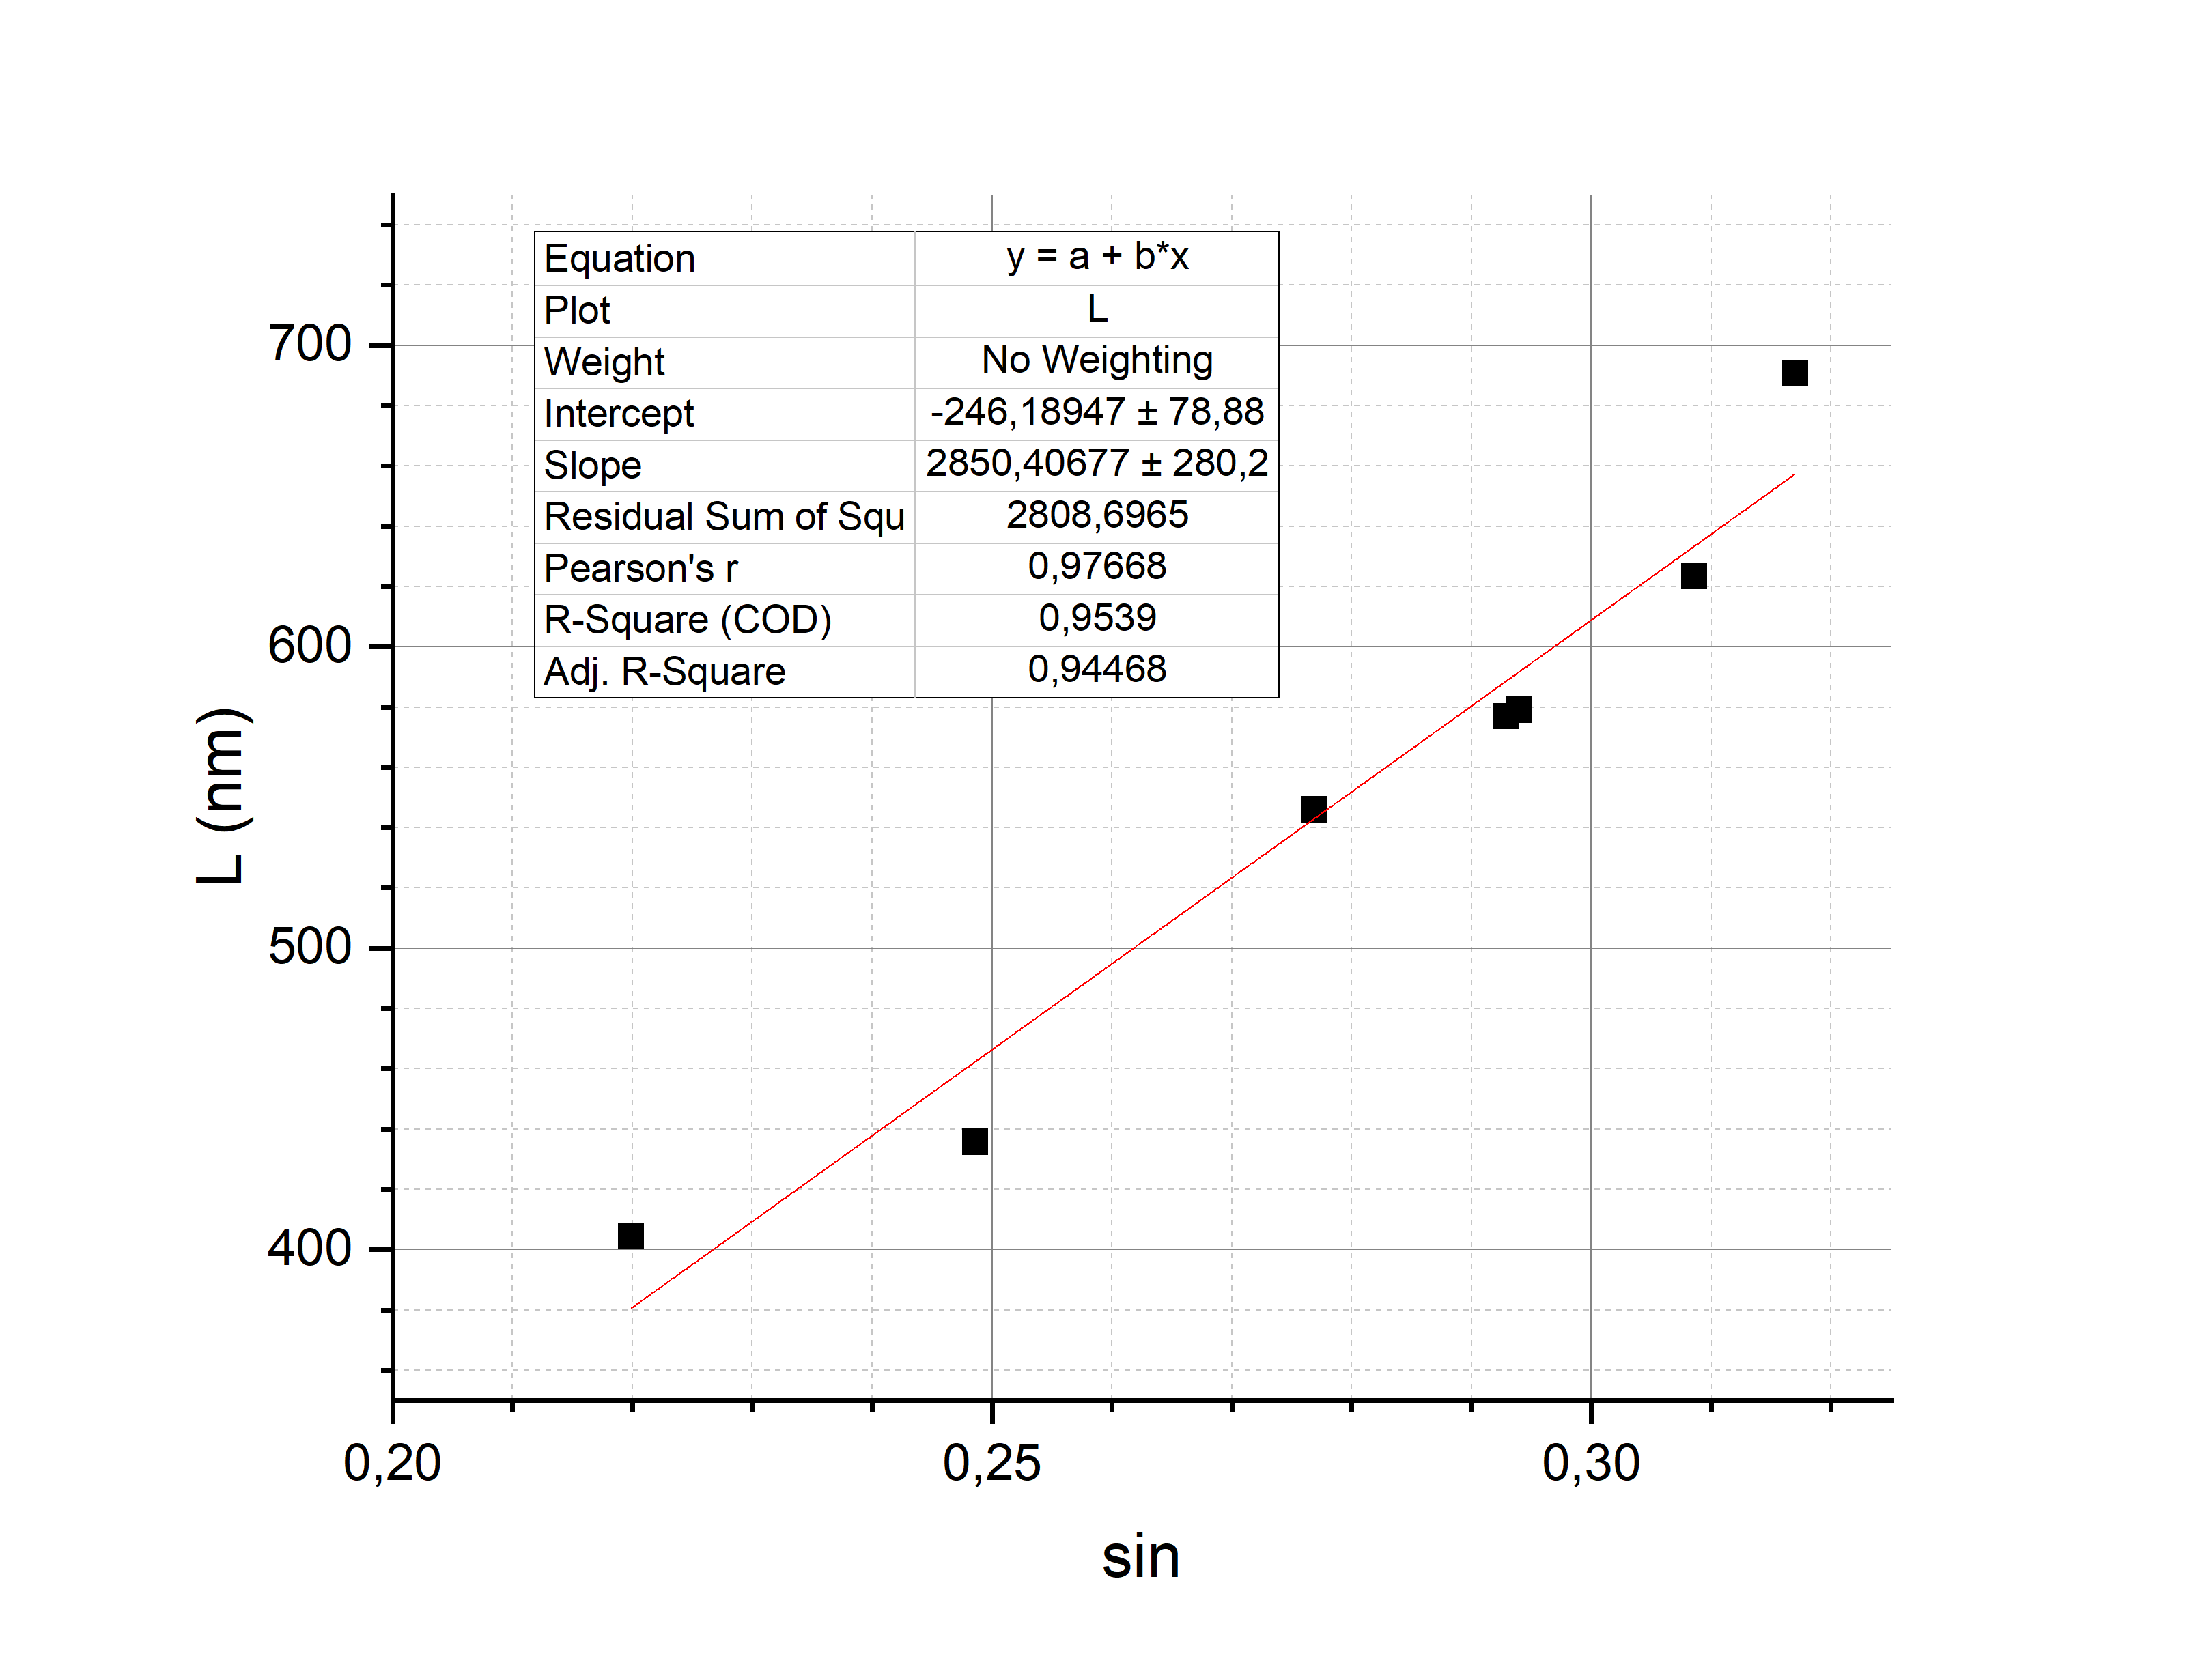
\includegraphics[width=0.9\textwidth]{gr1}
\end{center}
\ECaption{График зависимости $\lambda(\sin \varphi_n)$. Точки не совсем точно ложаться на прямую, скорее всего из-за того, что начало отсчета немного сбивалось при настройке на следующую полосу спектра.}
\end{figure}                             

Таким образом получено экспериментальное значение периода решетки:
\[d = 2850\pm 280\text{ нм.}\]

\subsection*{Угловая дисперсия}

Для оценки угловой дисперсии спектра, были определены угловые координаты желтой пары во всех видимых порядках. Тогда дисперсия рассчитывается по этой формуле:
\begin{equation}
D = \dfrac{\Delta\varphi}{\Delta\lambda},
\end{equation}
где $\Delta\lambda = 21$ ангстрем.

Тогда в зависимости от порядка, разницы координат желтой пары представлены на таблице 3. Так же в этой таблице рассчитаны значения угловой дисперсии теоретическим (2) и экспериментальным способом.

\begin{table}[h!]
\begin{center}
\begin{tabular}{|c|c|c|c|}
\hline
\rowcolor[HTML]{9698ED} 
m  & $\Delta\varphi$, s & $D_{\text{exp}}$, $\frac{s}{A^{\circ}}$ & $D_{\text{teor}}$, $\frac{s}{A^{\circ}}$ \\ \hline
-3 & 997   & 47.47 & 47.7  \\ \hline
\rowcolor[HTML]{9698ED} 
-2 & 512   & 24.38 & 27.62  \\ \hline
-1 & 243   & 11.57 & 12.89 \\ \hline
\rowcolor[HTML]{9698ED} 
1  & 225   & 10.71 & 12.89 \\ \hline
2  & 642   & 30.57 & 27.62  \\ \hline
\end{tabular}
\ECaption{Разность угловых координат желтой пары во всех видимых порядках (в угловых секундах).}
\end{center}
\end{table}

Далее на рис 5 представлен график зависимости дисперсии от порядка. На нем изображены оба способа рассчета угловой дисперсии.

\begin{figure}[h!]
\begin{center}
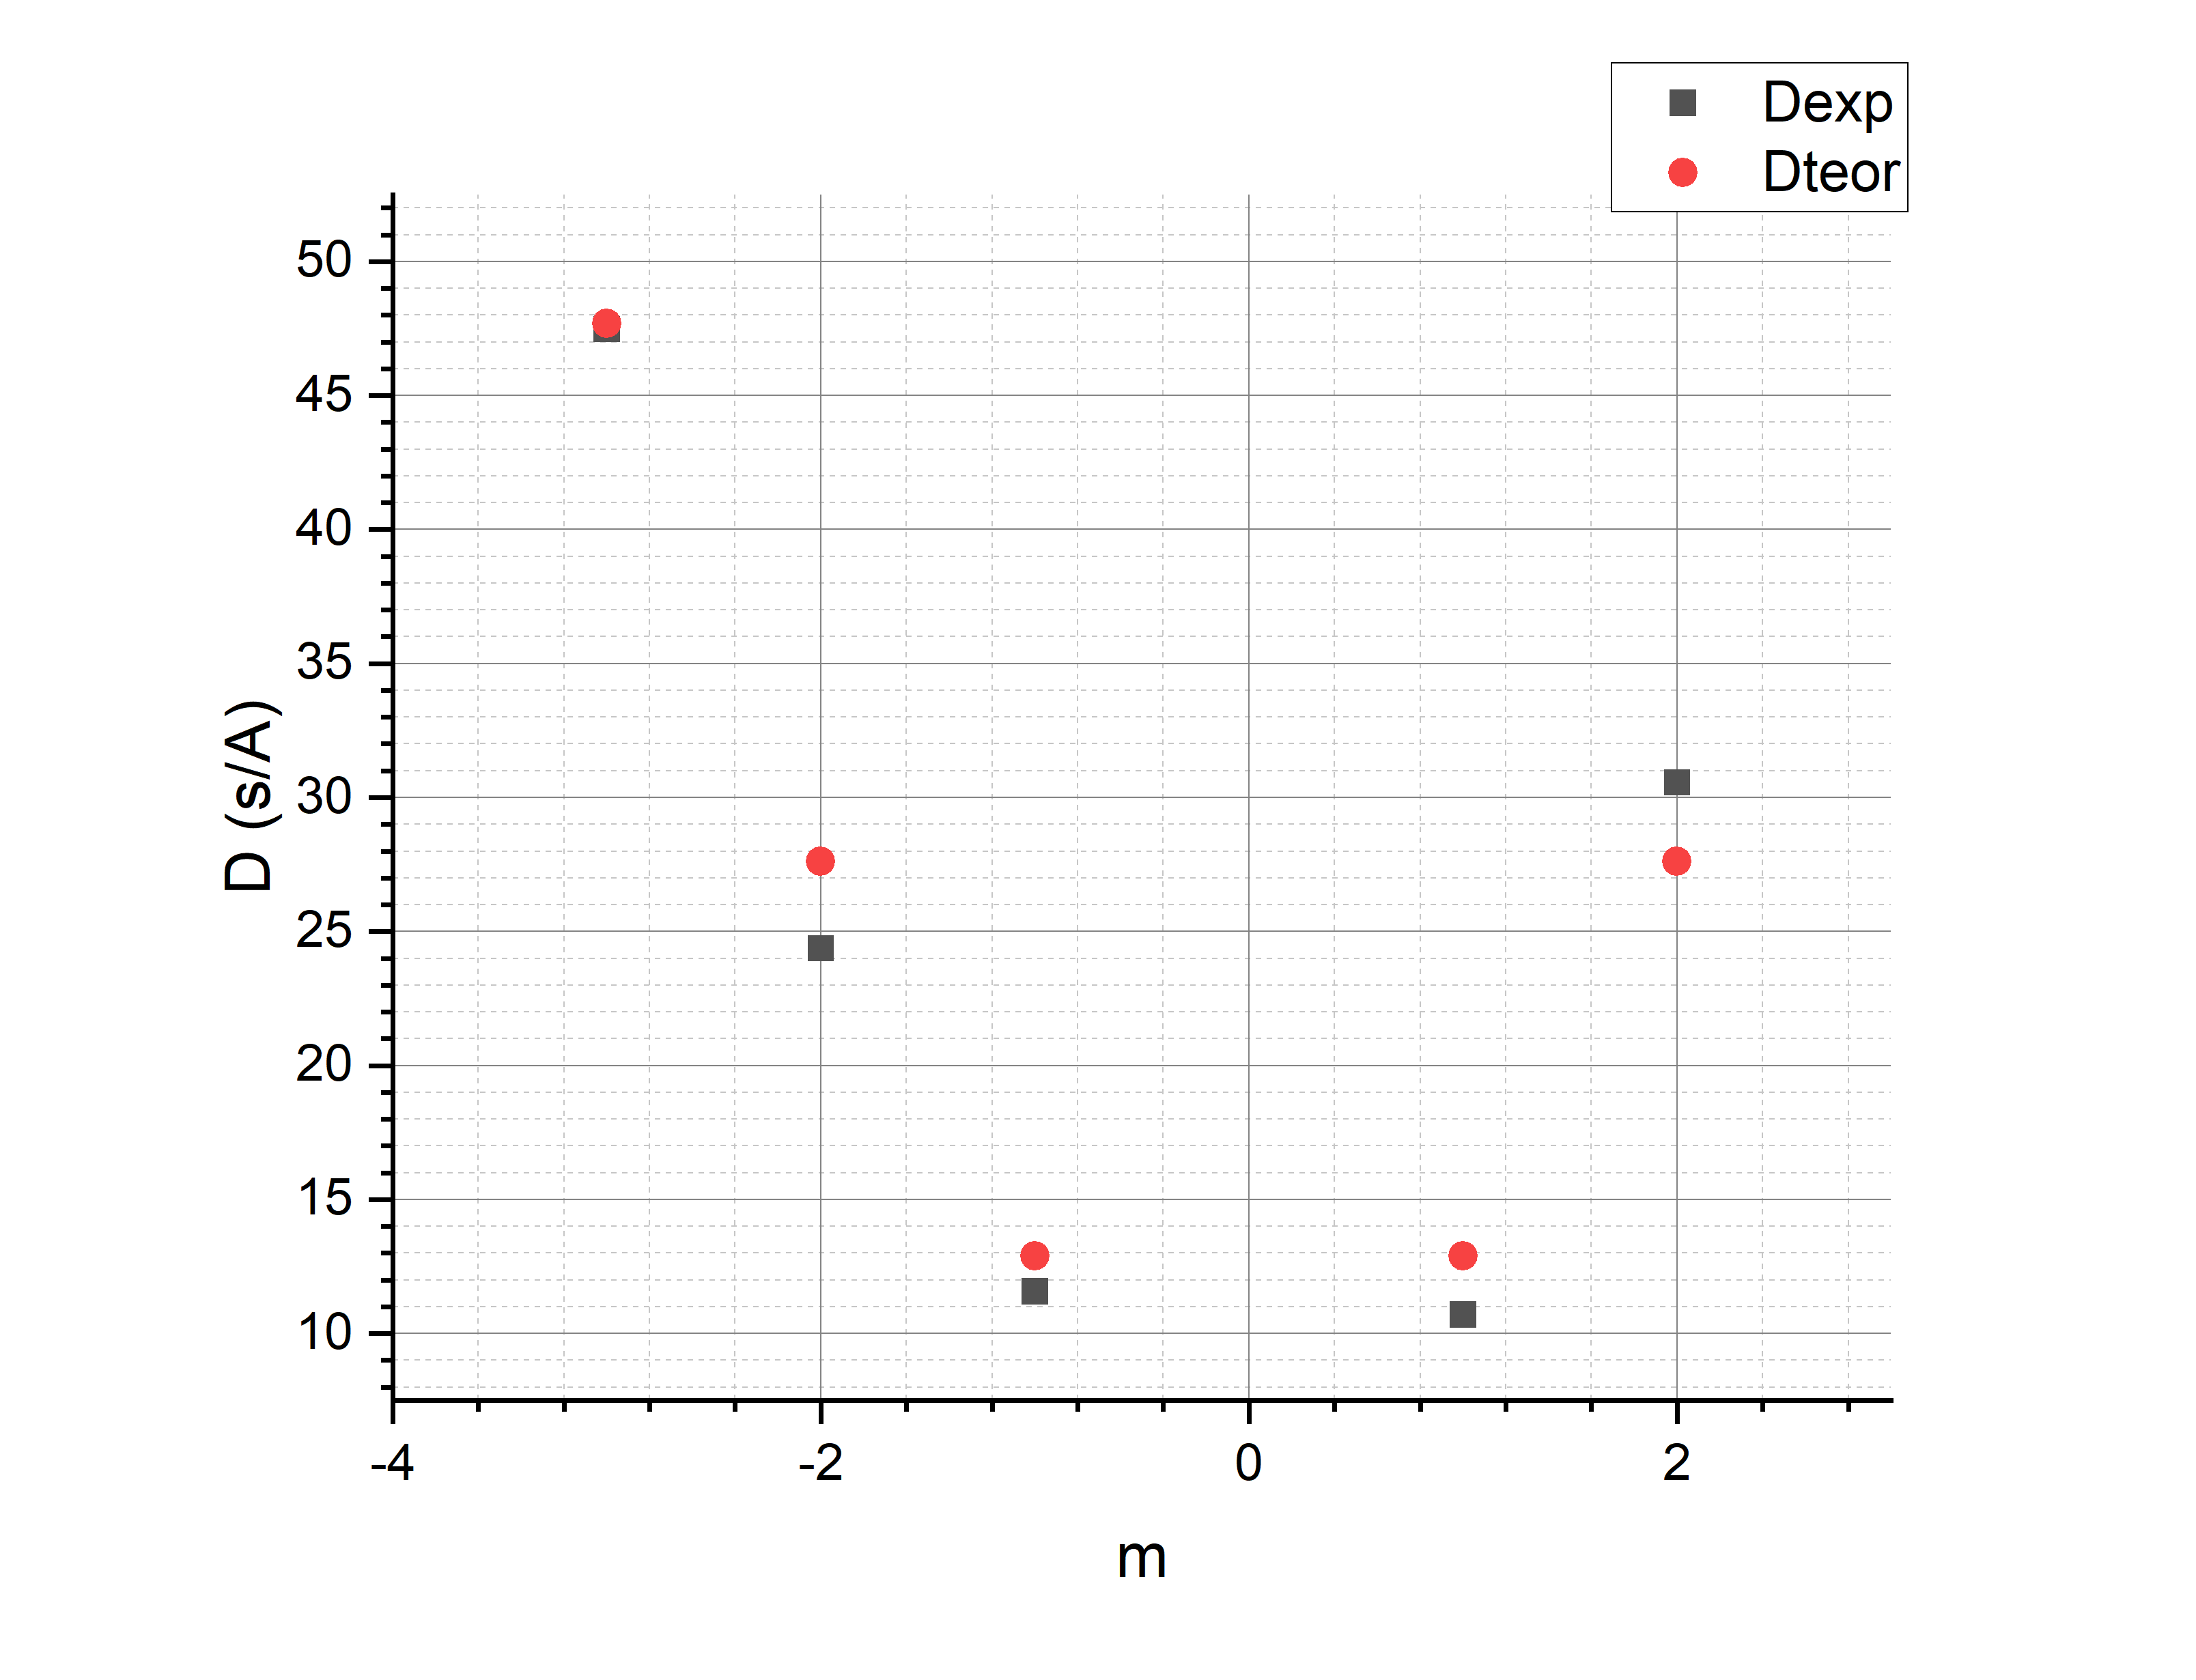
\includegraphics[width=0.9\textwidth]{gr2}
\end{center}
\ECaption{График зависимости $D(m)$. Экспериментальные точки изображены в форме квадратиков, а теоретические - кружочков.}
\end{figure} 

\subsection*{Разрешаюшая способность}

Чтобы рассчитать экспериментальную разрешающую способность (5), была измерена угловая ширина первой желтой линии 1 порядка спектра в угловых секундах:
\[\delta\varphi = 37''\]
Таким образом, зная её угловую координату получаем разрешающую способность:
\[R = \frac{\varphi}{\delta\varphi} = 1660.\]
\newpage
\section*{Вывод}

В процессе работы был исследован спектр ртутной лампы. На основании определения угловых координат полос спектра ртути был экспериментально рассчитан период дифракционной решетки, составивший $2850\pm 280$ нм, что является достаточно достоверным результатом с приемлимой точностью.

Далее, используя это значение $d$ была рассчитана угловая дисперсия спектра на основе желтой пары для разных периодов. Как показывает график, теоретические расчеты неплохо согласуются с экспериментом, что так же доказывает достоверность полученного ранее результата. 

И, наконец, экспериментально рассчитана разрешающая способность решетки. В результате получаем число эффективно работающих штрихов решетки $N = 1660$. На основании этого получаем, что размер освещенной части решетки равен примерно 5 мм, что согласуется с качественной оценкой.































\end{document}